% per commentare una riga mettere % al suo inizio
% per s-commentare una riga (ossia attivarla) togliere il % al suo inizio
%
\documentclass[cucitura%lascia margine per la rilegatura
%,twoside% per stampa fronte-retro (fortemente consigliato per tesi voluminose, opzionale per le altre)
,12pt% font più grande (12pt) rispetto a quello normalmente usato (11pt)
]{toptesi}
%
% Cambiare encoding a piacere; oppure non caricare nessun encoding se si usano
% solo caratteri a 7 bit (ASCII) nei file d'entrata.
%
\usepackage[a-1b]{pdfx}% formato PDF/A, obbligatorio per l'archiviazione delle tesi di Polito
\usepackage[utf8]{inputenc}% IMPORTANTE! usare codifica UTF-8 per le lettere accentate
\usepackage{amsmath, amssymb}
\usepackage{nccmath}
\usepackage{appendix}
\usepackage{longtable}
\usepackage{lscape}
\usepackage{adjustbox}
\usepackage{float}
\usepackage{accsupp}
%
% Commentare le righe seguenti se NON si è specificata l'opzione "pdfa"
\hypersetup{%
    pdfpagemode={UseOutlines},
    bookmarksopen,
    pdfstartview={FitH},
    colorlinks,
    linkcolor={blue},
    citecolor={red},
    urlcolor={blue}
  }
% \documentclass[11pt,twoside,oldstyle,autoretitolo,classica,greek]{toptesi}
% \usepackage[or]{teubner}
%%%%%%%%%%%%%%%%%%%%%%%%%%%%%%%%%%%%%%%%%%%%%%%%%%%%
%


% per inserire uno spazio "fantasma" nella definizione di un'abbreviazione
\usepackage{xspace}

% per inserire un DOI senza problemi coi caratteri "strani" ivi presenti
\usepackage{doi}
\renewcommand{\doitext}{DOI }% originally was "doi:"

% per inserire correttamente le unità di misura SI (incluse quelle binarie)
\usepackage[binary-units]{siunitx}
% se si desidera usare / invece che la potenza -1 per indicare "al secondo"
\sisetup{per-mode=symbol}

% per inserire codice di programmazione complesso
\usepackage{listings}% per inserire codice di programmazione complesso
\lstset{
basicstyle=\ttfamily,
columns=fullflexible,
xleftmargin=3ex,
numbers=none,
breaklines,
breakatwhitespace,
escapechar=`
}

% modify some page parameters
\setlength{\parskip}{\medskipamount}
\advance\voffset -5mm
\advance\textheight 30mm

% riga orizzontale
\newcommand{\HRule}{\rule{\linewidth}{0.2mm}}
% esempio di creazione di semplici abbreviazioni
\newcommand{\ltx}{\LaTeX\xspace}
\newcommand{\txw}{TeXworks\xspace}
\newcommand{\mik}{MikTex\xspace}
\newcommand{\html}{HTML\xspace}
\newcommand{\xhtml}{XHTML\xspace}

% esempio di creazione di un'abbreviazione con un parametro (il cui uso è indicato da #1)
\newcommand{\cmd}[1]{\texttt{#1}\xspace}
% per citare un RFC, es. \rfc{822}
\newcommand{\rfc}[1]{RFC-#1\xspace}
% per citare un file (es. \file{autoexec.bat}) o una URI fittizia (es. \file{http://www.lioy.it/})
% per le URI vere usare \url o \href
\newcommand{\file}[1]{\texttt{#1}\xspace}
% per inserire codice di esempio in-line
\newcommand{\code}[1]{\lstinline|#1|}
% importante per i pathname Windows perché non si può usare \ essendo un carattere riservato di Latex
\newcommand{\bs}{\textbackslash}
% definizione di un termine: formattazione ed inserimento nell'indice
\newcommand{\tdef}[1]{\textit{#1}\index{#1}}
% meta-termine, usato tipicamente nelle definizioni dei tag
\newcommand{\meta}[1]{\textit{#1}}


\definecolor{blond}{rgb}{0.98, 0.94, 0.75}
\definecolor{gray}{rgb}{0.4,0.4,0.4}
\definecolor{darkblue}{rgb}{0.0,0.0,0.6}
\definecolor{cyan}{rgb}{0.0,0.6,0.6}
\definecolor{Maroon}{rgb}{0.5,0.0,0.0}
\definecolor{darkgreen}{rgb}{0.0,0.5,0.0}

%\ExtendCaptions{english}{Abstract}{Acknowledgements}

\lstset{
	numbers=none, 
	numberstyle=\small, 
	numbersep=8pt, 
	frame = single, 
	framexleftmargin=20pt
}

\lstdefinelanguage{XML}
{
	backgroundcolor = \color{blond},
	basicstyle=\ttfamily\footnotesize,
	morestring=[b]",
	moredelim=[s][\bfseries\color{Maroon}]{<}{\ },
	moredelim=[s][\bfseries\color{Maroon}]{</}{>},
	moredelim=[l][\bfseries\color{Maroon}]{/>},
	moredelim=[l][\bfseries\color{Maroon}]{>},
	morecomment=[s]{<?}{?>},
	morecomment=[s]{<!--}{-->},
	commentstyle=\color{DarkOliveGreen},
	stringstyle=\color{blue},
	identifierstyle=\color{red}
}



\begin{document}
%\renewcommand{\lapagina}{\Roman{page}}
\english

\iflanguage{english}{%
	\retrofrontespizio{This work is subject to the Creative Commons Licence}
	\DottoratoIn{PhD Course in\space}
	\CorsoDiLaureaIn{Master of Science in\space}
	\NomeMonografia{Bachelor Degree Final Work}
	\TesiDiLaurea{Master Degree Thesis}
	\NomeDissertazione{PhD Dissertation}
	\InName{in}
	\CandidateName{Candidate}
	\AdvisorName{Supervisors}
	\TutorName{Tutor}
	\NomeTutoreAziendale{Internship Tutor}
	\CycleName{cycle}
	\NomePrimoTomo{First volume}
	\NomeSecondoTomo{Second Volume}
	\NomeTerzoTomo{Third Volume}
	\NomeQuartoTomo{Fourth Volume}
	\logosede[6cm]{PolitoLogo3}% or comma separated list of logos
}{}

\ateneo{}

%%% scegliere la propria facoltà (solo PRIMA dell'AA 2012-2013)
%
%\facolta[III]{Ingegneria dell'Informazione}
%\facolta[IV]{Organizzazione d'Impresa\\e Ingegneria Gestionale}
%\Materia{Remote sensing}% uso sconsigliato

%\monografia{Gestione informatizzata di un magazzino ricambi}% per la laurea triennale
\titolo{Prova}% per la laurea quinquennale e il dottorato
%\sottotitolo{Metodo dei satelliti medicei}% NON obbligatorio, per la laurea quinquennale e il dottorato

\corsodilaurea{Computer Engineering}% per la laurea di primo e secondo livello

\candidato{Benito \textsc{Marra}}% per tutti i percorsi
\relatore{prof.\ Fulvio Valenza}% per la laurea e il dottorato
\secondorelatore{prof.\  Name Surname}% per la laurea magistrale
\terzorelatore{\tabular[t]{@{}l}
	dott.  Name Surname\\[2pt]dott.  Name Surname
	\endtabular}% per la laurea magistrale
%\sedutadilaurea{Agosto 1615}% per la laurea quinquennale
%\sedutadilaurea{\textsc{July} 2019}% per la laurea triennale
\sedutadilaurea{\textsc{Academic~Year} 2023-2024}% per la laurea magistrale
%\annoaccademico{1615-1616}% solo con l'opzione classica
%\annoaccademico{2006-2007}% idem

%\logosede{logopolito}
%
%\chapterbib %solo per vedere che cosa succede; e' preferibile comporre una sola bibliografia
%\AdvisorName{Supervisors}
%\newtheorem{osservazione}{Osservazione}% Standard LaTeX


\hypersetup{
   pdfpagemode={UseOutlines},
   bookmarksopen,
    pdfstartview={FitH},
    colorlinks,
    linkcolor={blue},
    citecolor={green},
    urlcolor={blue}
  }

%
% per numerare e far comparire nell'indice anche le sezioni di quarto livello
%\setcounter{secnumdepth}{4}% section-numbering-depth
%\setcounter{tocdepth}{4}% TOC-numbering-depth (TOC=Table-Of-nt)

%\setbindingcorrection{3mm}

\errorcontextlines=9

\expandafter\ifx\csname StileTrieste\endcsname\relax
    \frontespizio
\else
    \paginavuota
    \tomo
\fi




\sommario


Text of the summary 



\ringraziamenti

Acknowledgement (optional)

%% inserire sempre nella tesi per la laurea di I livello, perché il nome dei tutori non è indicato sul frontespizio.
%Il lavoro descritto in questa monografia è stato svolto sotto la supervisione
%del Prof. Antonio Lioy (tutore accademico)% inserire sempre il nome del tutore accademico
% e dell'Ing. Mario Rossi (tutore aziendale)% inserire solo se la monografia è relativa ad un tirocinio.
%.

%\tablespagetrue % normalmente questa riga non serve ed e' commentata
%\figurespagetrue % normalmente questa riga non serve ed e' commentata

\indici

\listoffigures

\listoftables

\addcontentsline{toc}{chapter}{Listings}
\lstlistoflistings

\clearpage\pagestyle{empty}\mbox{}\clearpage

%\renewcommand{\lapagina}{\arabic{page}}

\mainmatter


\chapter{Introduction} \label{ch:intro}

\section{Thesis objective} 

Benvenuti alla mia tesi figli di puttana!

\section{Thesis description}

description \cite{noms2020}
%other chapters
\lstdefinestyle{mystyle}{
    backgroundcolor=\color{myyellow},
    basicstyle=\ttfamily\small,
    breaklines=true,
    frame=single,
    language=XML
}


\chapter{Network Security Automation e Verefoo} \label{ch:verefoo}




Nel mondo odierno le reti internet hanno rivestito un'importanza sempre maggiore, evolvendosi da piccole e semplici scenari per reti private domestiche
a grandi e complicate topologie per le aziende e la comunicazione in tutto il mondo. Trattandosi di un mondo sempre in evoluzione, anche la configurazione e
l'installazione di queste reti è diventata sempre più complessa, tanto da far notare sempre di più l'errore umano nelle impostazioni delle rete.
Per queste situazioni nasce l'idea di \textit{Network Security Automation}, che pone come obiettivo principale quello di riuscire a rendere la sicurezza delle reti
il più possibile autonoma, riducendo la possibilità di errore umano e delegando all'automatizzazione tutte le criticità della configurazione delle varie funzioni di rete.\\
In questo capitolo si introduce la definizione di \textbf{\textit{Security Function Chain (SFC)}} specificando la loro capacità nel migliorare la sicurezza delle reti,
successivamente verrà introdotto il framework Verefoo che utilizza le SFC per poter produrre delle topologie di rete robuste e sicure e automatizzare il processo di creazione e configurazione delle reti.\\
L'ultima sezione del capitolo infine spazia sugli input che il framework accetta, le \textit{Network Security Functions (NSFs)}, cioè tutte le funzioni che la rete deve rispettare come ad esempio filtrare dei pacchetti
o criptare del traffico dati. 


\section{Service Function Chain} 

All'interno delle reti è possibile far passare il traffico in maniera \textit{End-to-End, Site-to-Site o End-to-Site}.
Durante la comunicazione nelle reti moderne è solito far transitare i pacchetti attraverso nodi che si occupano di funzioni specifiche all'interno della
rete (Ad esempio un Packet Filter o un Network Address Translator NAT), che sono necessari per poter far rispettare alla rete determinate caratteristiche l'utente richiede.
I nodi che sono adibiti a svolgere le funzioni prendono il nome di \textit{Service Function (SF)} ed il collegamento di più nodi adibiti a SF viene definito 
\textit{Service Function Chain (SFC)}. Una definizione formale di SF e SFC è stata presentata nel RFC 7665 \cite{rfc7665} 
che definisce le seguenti:

\begin{itemize}
    \item \textbf{Service Function}: Una funzione che è responsabile del trattamento specifico dei pacchetti ricevuti. Una Service Function può agire su varie livelli di uno stack di protocollo (ad esempio, al livello di rete o ad altri livelli OSI). 
    Come componente logica, una SF può essere realizzata come un elemento virtuale o essere incorporata in un elemento di rete fisico.
     Una o più SF possono essere incorporate nello stesso elemento di rete. Possono esistere più occorrenze della funzione di servizio nello stesso dominio amministrativo.
    \item \textbf{Service Function Chain} Una Service Function Chain definisce un insieme ordinato di funzioni di servizio astratte e vincoli di ordinamento che devono essere applicati a pacchetti e/o frame e/o flussi selezionati come risultato di una classificazione. 
    Un esempio di una Service Function astratta è un "firewall". 
    L'ordine implicito potrebbe non essere una progressione lineare poiché l'architettura consente SFC che si ramificano su più di un percorso e consente anche casi in cui c'è flessibilità nell'ordine in cui le Service Function devono essere applicate. 
\end{itemize}

La possibilità di definire SF separate e di combinarle fra loro nell'ordine che si preferisce garantisce alle reti la possibilità di essere flessibili e scalabili facilmente.
Come infatti è descritto dalla definizione di SFC la concatenazione di più SFC permette ramificazioni su più percorsi, garantendo molteplici comunicazioni fra due host con carateristiche di sicurezza differenti.
Per comprendere meglio il concetto di SFC, un esempio fornito è il seguente:


\begin{figure}[h]  % 'h' significa che la figura viene posizionata qui
    \centering
    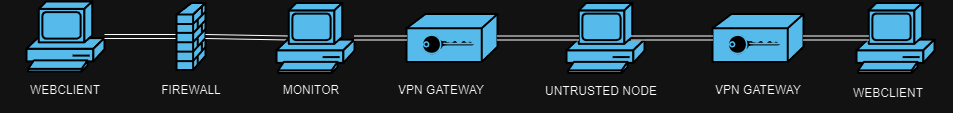
\includegraphics[width=1\textwidth]{SFC.png}  % Sostituisci 'nome_immagine' con il nome del tuo file immagine e l'estensione
    \caption{Esempio di Service Function Chain}
    \label{fig:esempio}
  \end{figure}


Come si può notare, vi sono diversi elementi all'interno di questo esempio.
Per quanto riguarda i vari SF possiamo trovare i seguenti:

\begin{itemize}
    \item \textbf{Firewall}: Si occupa di fare da packet filter fra i due webclient, per filtrare solo i pacchetti che effettivamente sono necessari alla comunicazione
    \item \textbf{Monitor}: Si occupa di monitorare il traffico in transito fra i due nodi, può essere un nodo da interrogare in caso di problematiche all'interno della rete per controllare che il firewall svolga il suo ruolo correttamente.
    \item \textbf{VPN Gateway}: Si occupa di criptare e decriptare il traffico. In questa topologia è fondamentale la loro presenza in quanto vi è un nodo considerato non affidabile, di conseguenza tutte le comunicazioni che passano attraverso quel nodo sono criptografate.
\end{itemize}

L'unione dei tre SF in questo specifico ordine definice una Service Function Chain. E' importante notare che se l'ordine fosse stato diverso (ad esempio mettendo prima i 2 VPN Gateway e dopo il firewall)
la SFC risultante sarebbe stata diversa da quella di partenza, garantendo una ramificazione.

\section{Verefoo}
\subsection{Introduzione}
 Il potenziamento progressivo delle tecnologie appena descritte ha portato rapidamente allo sviluppo di reti  che automatizzavano i lavori di configurazione che solitamente venivano svolti manualmente.
 Un esempio di queste nuove tecnologie viene svolto da VEREFOO\cite{Bringhenti2019}(VErified REfinement and Optimized Orchestration), un framework che si pone diversi obiettivi fra i quali la definizione
ad alto livello dei requisiti di sicurezza di rete, l'allocazione automatica ed ottimale delle varie Service Function per ottenere la maggior efficenza di rete allocando le minori risorse possibili, e la
configurazione automatica delle varie \textit{Network Security Functions}, eliminando l'errore  umano che in reti di grandi dimensioni è solito capitare.
Come è possibile intuire, la sfida di produrre una rete configurata automaticamente e correttamente è molto difficile da ottenere, perciò per assicurare la correttezza formale dei risultati ottenuti da Verefoo
l'intero framework utilizza un metodo formale che si basa sulla risoluzione di un \textit{Maximum Satisfiability Modulo Theories} (MaxSMT) tramite l'engine Z3 di Microsoft.\\
Questo, essendo basato su 3 pilastri quali \textit{Ottimizzazione, Ottimalità e Correttezza Formale}, Verefoo si pone 2 obiettivi da soddisfare:

\begin{enumerate}
    \item L'allocazione ottimale dei vari NSFs
    \item La configurazione ottimale dei vari NSFs.
\end{enumerate}

\subsection{Descrizione del modello}
Il modello di Verefoo, descritto in figura 2.2 richiede in input due elementi fondamentali:

\begin{itemize}
    \item \textbf{Service Graph}: Una topologia logica delle funzioni della rete che insieme formano un collegamento end-to-end. A differenza delle SFC il Service Graph può avere diversi percorsi per collegare due punti nella rete
    presentando la ramificazione tipica della concatenazione di SFC. Durante la creazione del Service Graph non è necessario specificare nessun requisito di sicurezza, come ad esempio Firewall, Monitors o Filtering Databases. 
    \item \textbf{Network Security Requirements}: Sono i requisiti di sicurezza che la rete in output dovrà avere dopo la computazione di Verefoo. Questo elemento è fondamentale per costruire il modello di MaxSMT da risolvere tramite Z3.
    Allo stato attuale, Verefoo consente di avere 3 requisiti di sicurezza principali:
        \begin{enumerate}
            \item \textbf{Reachability Property}: Indica che un nodo Y di destinazione deve essere raggiungibile da un nodo di partenza X in almeno un percoso della topologia.
            \item \textbf{Isolation Property}: Indica che un nodo Y di destinazione \textbf{NON} deve essere raggiungibile da un nodo di partenza X in tutti i possibili percorsi all'interno della topologia.
            \item \textbf{Protection Property}: Indica che la comunicazone tra un nodo di partenza X ed un nodo di destinazione Y deve essere sicura. In questo requisito è anche possibile specificare
                un nodo definito \textit{"Untrusted Node"} ovvero un nodo che potrebbe essere un possibile punto di debolezza nella rete e che quindi deve poter vedere solo il traffico criptografato.
        \end{enumerate}
\end{itemize}


\begin{figure}[h]  % 'h' significa che la figura viene posizionata qui
    \centering
    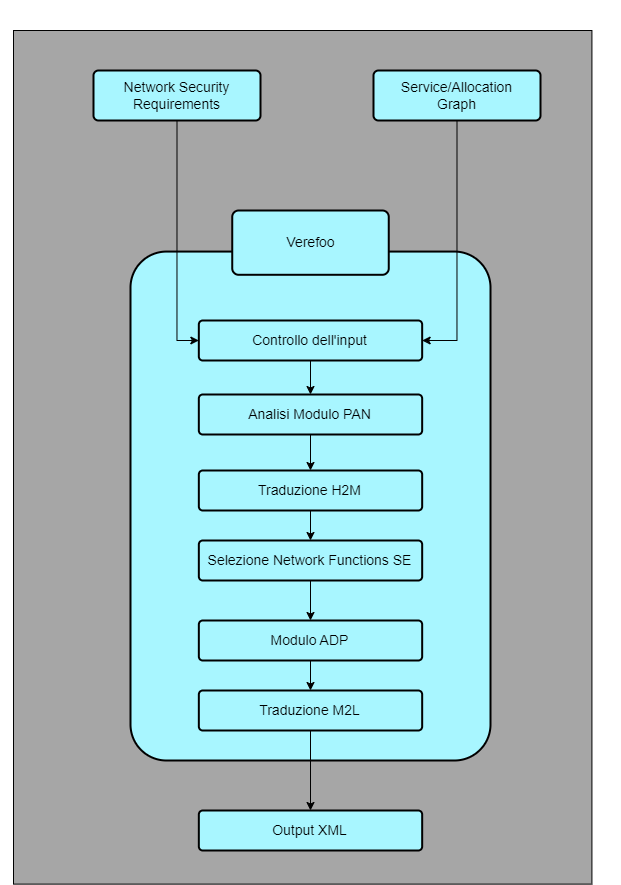
\includegraphics[width=1\textwidth]{VerefooArchitecture.png}  % Sostituisci 'nome_immagine' con il nome del tuo file immagine e l'estensione
    \caption{Architettura di VEREFOO \cite{Bringhenti2019}}
    \label{fig:architettura_verefoo}
  \end{figure}

Successivamente all'input, il framework esegue una serie di passi che possono essere così riassunti:

\begin{enumerate}
    \item \textbf{Fase di controllo dell'input}: In questa fase Verefoo accetta l'input passato sotto forma di file XML e controlla la coerenza dell'input fornito. Il framework 
         oltre ad accettare l'input composto da Service Graph e NSRs accetta anche la possibilità di fornire un \textit{Allocation Graph} al posto del Service Graph(figura 2.3). La
         differenza fondamentale fra i due è che nel secondo oltre ai vari nodi della rete descritti nel Service Graph si specificano anche dei nodi aggiuntivi, chiamati \textit{Allocation Places}
         che rappresentano i punti nella topologia dove è possibile istanziare una funzione di sicurezza di rete.
    \item \textbf{Fase di analisi del modulo PAN}: qui Verefoo esegue un'analisi delle policy che sono state passate in input. Più specificatamente viene controllato che i vari NSRs siano coerenti fra
    loro, evidenziando eventuali errori (ad esempio non si può avere una Reachability Property ed una Isolation Property con gli stessi nodi di partenza e destinazione). Alla fine dell'analisi delle policy
    viene prodotto il numero minimo di vincoli che devono essere rispettati affinchè la topologia soddisfi i NSRs richiesti. In caso di errore un report viene solitamente fornito in output per comprendere 
    il perchè un determinato input non è soddisfabile.
    \item \textbf{Trasformazione a Medium Level Language}: Una volta definiti ad alto livello i vincoli da far rispettare alla topologia, questi vengono tradotti da un linguaggio di alto livello
    ad uno di medio livello tramite il componente H2M. 
    \item  \textbf{Selezione delle Network Function}:Ricevuto l'output dal modulo H2M il modulo Network Functions Selection (SE) si occupa di selezionare da un catalogo le NSF necessarie a rispettare i requisiti
    di alto e medio livello. Questo catalogo è anche accessibile al designer della rete nella fase di design disponibile nella Service GUI di Verefoo.
    \item \textbf{Allocazione, Distribuzione e Piazzamento}:Durante questo passo del framework viene eseguito, come suggerito dal titolo, l'allocazione delle varie funzioni di rete calcolate tramite
    il modulo NF Selection e i vincoli di medio livello tradotti nell'H2M. Questo compito è affidato al modulo ADP che è il cuore di Verefoo, perchè decide in quali punti della rete e con quali configurazioni
    le varie NFs devono essere allocate. L'ADP produce quindi un nuovo Service Graph nel quale sono allocate anche le funzioni di sicurezza di rete, e produce dei file di configurazione per ciascuna funzione allocata
    nel nuovo Service Graph. Queste configurazioni sono create in un linguaggio di basso livello grazie al modulo M2L presente all'interno dell'ADP.
\end{enumerate}


\begin{figure}[h]  % 'h' significa che la figura viene posizionata qui
    \centering
    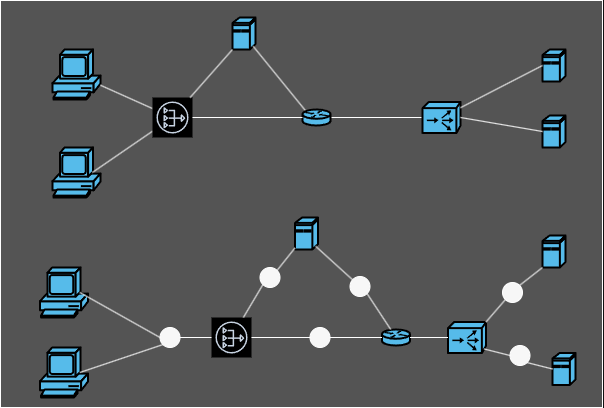
\includegraphics[width=0.9\textwidth]{Service_Allocation_Graph.png}  % Sostituisci 'nome_immagine' con il nome del tuo file immagine e l'estensione
    \caption{Esempi di Service (in alto) e Allocation(in basso) Graphs \cite{Bringhenti2019}}
    \label{fig:AllocationGraph}
  \end{figure}



\section{Definizione ed esempio di Grafo di servizio e di allocazione}

Il primo fondamentale input che deve essere fornito a Verefoo è il grafo di servizio o il grafo di allocazione. 
Viene definito fondamentale perchè è l'unico modo che ha il framework per comprendere la topologia di rete con la quale dovrà interfacciarsi per soddisfare le richieste dell'utente.
Allo stato attuale all'interno di Verefoo è possibile definire come SF le seguenti:

\begin{itemize}
    \item \textbf{Load Balancer}: è uno strumento di controllo di flusso della rete. Il load balancer è infatti in grado di distribuire il carico di lavoro in maniera equa nella rete
        evitando delle situazioni nelle quali alcuni collegamenti fra i nodi risultano sovraccaricati mentre altri inattivi. È quindi in grado di migliorare l'affidabilità e l'efficienza di
        un sistema distribuito.
    \item \textbf{Network Address Translator (NAT)}: è un servizio che consente la traduzione degli indirizzi IP tra due reti. Il suo obiettivo principale è consentire a dispositivi in una rete 
    privata di condividere un singolo indirizzo IP pubblico per accedere a risorse esterne su Internet.  
    \item \textbf{Web Client}: è un'applicazione software o un dispositivo che consente agli utenti di accedere a risorse e servizi su Internet utilizzando il protocollo HTTP (Hypertext Transfer Protocol) o il suo equivalente sicuro HTTPS (Hypertext Transfer Protocol Secure). 
    Questo tipo di client è progettato per interagire con i server web, recuperare informazioni e visualizzare contenuti web.
    \item \textbf{Web Server}: è un software o un'applicazione che fornisce risorse e servizi su Internet, rispondendo alle richieste provenienti dai web client. Il suo ruolo principale è accettare richieste HTTP (Hypertext Transfer Protocol) o HTTPS (Hypertext Transfer Protocol Secure) 
    da parte dei client e inviare loro le risorse richieste.
    \item  \textbf{Packet Filter(Firewall)}: è un componente di sicurezza della rete progettato per monitorare, analizzare e controllare il traffico di rete in base a regole predefinite. La sua funzione principale è quella di decidere quali pacchetti di dati possono attraversare il firewall e raggiungere la destinazione e quali devono essere bloccati.
    \item  \textbf{Web Cache}: è un meccanismo di memorizzazione temporanea che conserva copie di risorse web come pagine HTML, immagini, fogli di stile e altri contenuti multimediali. L'obiettivo principale della web cache è accelerare il caricamento delle pagine web e ridurre il carico sulla rete e sui server web, fornendo ai client risorse già memorizzate localmente anziché scaricarle nuovamente da Internet.
\end{itemize}

Questi elementi possono essere inseriti nella creazione di una rete da fornire a Verefoo. Il framework è in grado di accettare file XML che descrivono il grafo della topologia di rete definendo i nodi nel seguente modo:

\begin{itemize}
    \item \textbf{nome}: é l'indirizzo ip che caratterizza il nodo.
    \item \textbf{funzionalità}: descrive quale delle SF descritte precedentemente il nodo implementa.
    \item \textbf{nodi vicini}: viene fornita una lista di nodi adiacenti al nodo in questione definiti dal loro indirizzo IP. 
    \item  \textbf{configurazione}: viene specificata la configurazione, ove necessaria, per poter istanziare la funzionalità definita al campo precedente.
\end{itemize}


\newpage

\section{Definizione ed esempi delle proprietà di sicurezza}

Le proprietà di sicurezza sono il secondo input che può essere fornito a Verefoo per stabilire i vincoli necessari affinchè
si possa creare una rete sicura. A differenza del primo parametro di input, la definizione della proprietà di sicurezza è 
responsabilità dell'amministratore della rete, in quanto deve decidere tramite le possibilità offerte da Verefoo e dalla GUI ad esso associata
quante e quali proprietà inserire nella propria rete per garantire la sicurezza richiesta.\\
Per garantire flessibilità al framework è possibile inserire le definizioni sia con un linguaggio a basso livello definendo rispetti IP, porte e protocolli
da accettare o rifiutare che con un linguaggio ad alto livello nel quale i vari elementi della rete verranno definiti da dei numeri che poi saranno mappati a degli IP.

I requisiti prodotti all'interno di verefoo saranno formulati con la seguente definizione:

\begin{lstlisting}[caption={Definizione di una proprietà di sicurezza generica},float={h} , label=lst:securityRule]
    [ruleType, IPSrc, IPDst, portSrc, portDst, transportProto]
\end{lstlisting}

\begin{itemize}
    \item \textbf{ruleType}: specifica quale proprietà stiamo definendo. Allo stato attuale del framework ci sono 3 possibili opzione: Reachability Property, Isolation Property e Protection Property.
    \item \textbf{IPSrc}: indica l'indirizzo IP sorgente, cioè il primo nodo della rete dal quale il requisito deve essere applicato.
    \item \textbf{IPDst}: indica l'indirizzo IP destinazione, ovvero l'ultimo nodo della rete dal quale il requisito deve essere applicato.
    \item \textbf{portSrc}:specifica la porta di rete del nodo sorgente che il protocollo di trasporto utilizzerà per inoltrare i pacchetti di rete. In questa opzione è possibile 
        inserire il valore \textit{"*"} che rappresenterà il range di tutte le porte possibili.
    \item \textbf{portDst}:specifica la porta di rete del nodo destinazione che il protocollo di trasporto utilizzerà per ricevere i pacchetti di rete. Come per il valore 
        portSrc anche in questo caso è possibile inserire il valore \textit{"*"} per rappresentare tutte le possibili porte di destinazione.
    \item \textbf{transportProto}:è il campo che specifica quale protocollo di trasporto verrà utilizzato per soddisfare la regola. Allo stato attuale Verefoo consente di utilizzare 2 possibili protocolli, UDP e TCP.
\end{itemize}

\newpage

I campi IPSrc e IPDst non sono limitati a descrivere un singolo host sorgente e un singolo host destinazione per ogni requisito. È infatti possibile utilizzare i due campi per definire anche delle sottoreti. 
Il framework di Verefoo, infatti, definisce gli IP con la classica notazione decimale:

\begin{center}
    \centering  % Aggiunge il comando per centrare il testo
    \textit{ip= ip1.ip2.ip3.ip4}
\end{center}

Ogni elemento da ip1 a ip4 deve appartenere al range [0-255] oppure è possibile utilizzare il valore \textit{"*"} per definire l'intera sottorete.
Grazie a questa implementazione è possibile definire le sottoreti come ad esempio 40.5.0.0\textbackslash16 utilizzando la notazione 40.5.*.* o anche sottoreti
più piccole come 20.1.1.0\textbackslash24 scrivendo 20.1.1.* . \\

Di seguito viene fornita una descrizione più dettagliata dei vari requirements specificabili su Verefoo e di come il framework li traduca in requisiti più generali che la topologia
di rete deve avere affinchè si possa soddisfare la richiesta dell'utente.

\subsection{Reachability Requirements}

I requisiti di raggiungibilità sono definiti nel framework di Verefoo per garantire che un determinato Host sorgente che verrà definito Host-S sia 
in grado di comunicare in maniera diretta e definita con un host destinazione che verrà nominato Host-D. Per garantire ciò è necessario assicurarsi che tutti i 
packet filter presenti nella connessione fra Host-S ed Host-D non scartino mai i pacchetti di questa comunicazione. Per ottenere questo obiettivo è quindi possibile
configurare i packet filter della rete in due modalità: blacklist e whitelist. Nella prima i packet filter faranno transitare tutto il traffico tranne quello specificato
nelle regole definite, mentre nella seconda bloccherà tutto il traffico in entrata escluso quello specificato nelle regole che gli sono state imposte.

Per poter dare per certo che il requisito sia applicabile alla topologia Verefoo svolge le seguenti operazioni:

\begin{enumerate}
    \item  Viene svolto un controllo formale sulla definizione della regola, cioè viene controllata la correttezza di tutti i campi inseriti nella proprietà. In questa prima fase
        Verefoo controlla se gli input inseriti sono tutti presenti e definiti nella maniera corretta (Come ad esempio Stringhe e indirizzi ip come numeri decimali).
    \item Viene svolto un controllo logico sulla definizione della regola, cioè viene controllato che l'indirizzo IP sorgente e quello destinazione appartengano effettivamente a degli host definiti
        nella rete. Inoltre viene controllato anche il protocollo di trasporto, assicurandosi che sia UDP o TCP.
    \item Si ispeziona l'Host-S, e ci si assicura che sia possibile inoltrare il traffico destinato all'Host-D in almeno uno dei nodi adiacenti poichè è sufficiente garantire che esista almeno un percorso
        definito per la comunicazione fra Host-S e Host-D
    \item Infine viene attenzionato l'Host-D, sincerandosi che sia possibile ricevere il traffico proveniente dall'Host-S da almeno uno dei nodi adiacenti, perchè garantisce che almeno un percorso fra l'Host-S
    e l'Host-D sia stato trovato.
\end{enumerate}

Di seguito è possibile trovare un esempio svolto da Verefoo per soddisfare un requisito di raggiungibilità:\\
\begin{figure}[h]  % 'h' significa che la figura viene posizionata qui
    \centering
    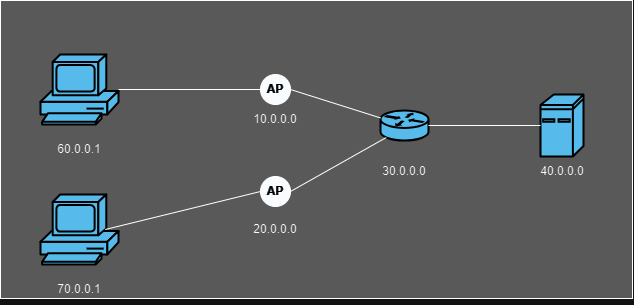
\includegraphics[width=0.8\textwidth]{Reachability.png}  % Sostituisci 'nome_immagine' con il nome del tuo file immagine e l'estensione
    \caption{Grafo di allocazione per requisito di raggiungibilità}
    \label{fig:Reachability}
  \end{figure}

Successivamente è necessario definire la definizione di requisito di raggiungibilità tra l'Host-S 60.0.01 e l'Host-D 40.0.0.0. Nel caso di questo esempio
proveremo a far comunicare i due Host tramite solo il protocollo TCP:
\begin{lstlisting}[style=mystyle,caption={Esempio di requisito di raggiungibilità}]
    <PropertyDefinition>
    <Property graph="0" name="ReachabilityProperty" src="60.0.0.1" dst="40.0.0.0" lv4proto="TCP" src_port="*" dst_port="*"/>
    </PropertyDefinition>
    \end{lstlisting}
    \newpage
Il risultato aspettato è il seguente:\\
\begin{figure}[h]  % 'h' significa che la figura viene posizionata qui
    \centering
    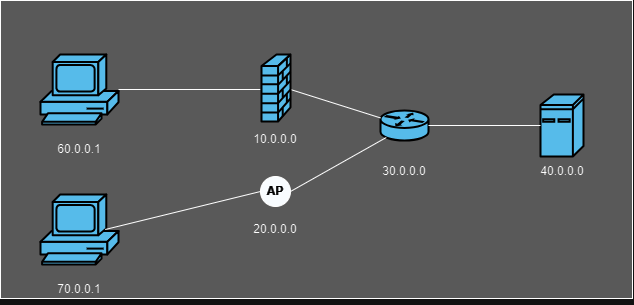
\includegraphics[width=0.8\textwidth]{Reachability_risolta.png}  % Sostituisci 'nome_immagine' con il nome del tuo file immagine e l'estensione
    \caption{Output grafo di esempio per requisito di raggiungibilità}
    \label{fig:Reachability_Soddisfatta}
  \end{figure}


Come si può notare, è stato posto un firewall che funge da packet filter che esclude tutte le comunicazioni uscenti da 60.0.0.1 e dirette a 40.0.0.0 che non utilizzano
il protocollo TCP. Il firewall è quindi stato impostato in blacklist mode negando tutto il traffico che non soddisfa la regola definita sopra.





\subsection{Isolation Requirements}

I requisiti di isolamento sono definiti nel framework di Verefoo per garantire
che un determinato Host sorgente che verrà definito Host-S non sia in grado di comu-
nicare in maniera diretta e definita con un host destinazione che verrà nominato
Host-D. Al fine di poter garantire ciò è necessario che tutti i packet filter presenti nel collegamento tra
Host-S e Host-D scartino a priori ogni pacchetto. In maniera equivalente ai requisiti di raggiungibilità è possibile
implementare nelle reti questo requisito tramite l'utilizzo di packet filter. Analogamente, sarà possibile impostare i
packet filter in blacklist, cioè bloccando solo le comunicazioni che vengono specificate dalle regole di filtraggio, oppure in 
whitelist, permettendo il transito solo dei pacchetti che fanno match con le regole di filtraggio.\\
Affinchè ciò sia implementato correttamente, Verefoo analizza ed opera nel seguente modo ogni requisito di isolamento ricevuto:

\begin{enumerate}
    \item  Come per i requisiti di raggiungibilità, viene svolto un controllo formale sulla definizione della regola, cioè viene controllata la correttezza di tutti i campi inseriti nella proprietà. In questa prima fase
        Verefoo controlla se gli input inseriti sono tutti presenti e definiti nella maniera corretta (Come ad esempio Stringhe e indirizzi ip come numeri decimali).
    \item Viene svolto un controllo logico sulla definizione della regola, cioè viene controllato che l'indirizzo IP sorgente e quello destinazione appartengano effettivamente a degli host definiti
        nella rete. Inoltre viene controllato anche il protocollo di trasporto, assicurandosi che sia UDP o TCP.
    \item Si ispeziona l'Host-S, e ci si assicura che sia possibile inoltrare il traffico destinato all'Host-D in almeno uno dei nodi adiacenti poichè è sufficiente garantire che esista almeno un percorso
        definito per la comunicazione fra Host-S e Host-D
    \item Infine viene attenzionato l'Host-D, sincerandosi che non sia possibile ricevere il traffico proveniente dall'Host-S da nessuno dei nodi adiacenti, così da garantire che non esiste nessun percorso in grado di
    far comunicare l'Host-S e l'Host-D.
\end{enumerate}

Al fine di poter portare all'attenzione un esempio di questo requisito di sicurezza, si utilizzerà la stessa topologia di rete 
consultabile nell'immagine \ref{fig:Reachability}.\\
A differenza del requisito di raggiungibilità, in questo caso la definizione sarà la seguente:\\

\begin{lstlisting}[style=mystyle,caption={Esempio di requisito di isolamento}]
    <PropertyDefinition>
    <Property graph="0" name="IsolationProperty" src="70.0.0.1" dst="40.0.0.0" lv4proto="UDP" />    </PropertyDefinition>
    \end{lstlisting}

In questo caso viene espresso che tutto il traffico proveniente dall'Host-S 70.0.0.1 e diretto all'Host-D 40.0.0.0 che transita
tramite il protocollo di livello 4 UDP, deve essere bloccato e quindi non arrivare a destinazione.
La computazione svolta da Verefoo porta alla seguente:

\begin{figure}[h]  % 'h' significa che la figura viene posizionata qui
    \centering
    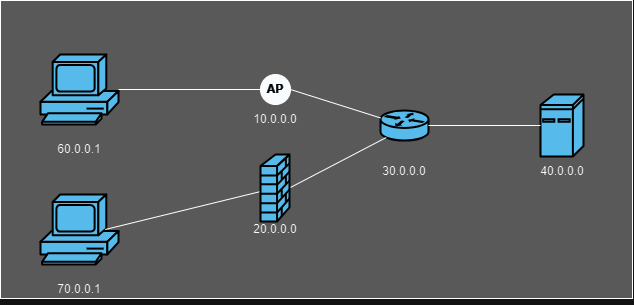
\includegraphics[width=0.8\textwidth]{Isolation_Soddisfatta.png}  % Sostituisci 'nome_immagine' con il nome del tuo file immagine e l'estensione
    \caption{Output grafo di esempio per requisito di isolamento}
    \label{fig:Isolation_Soddisfatta}
  \end{figure}

  A differenza della \ref{fig:Reachability_Soddisfatta}, il packet filter allocato da Verefoo è stato impostato in blacklist
  mode. Facendo ciò le comunicazioni fra i due host 70.0.0.1 e 60.0.0.1 sono ancora garantite e l'unica regola che blocca il traffico
  dati è specifica per le comunicazioni in UDP da 70.0.0.1 a 40.0.0.0.
  \newpage


  \subsection{Protection Requirements}
  I requisiti di protezione sono definiti nel framework di Verefoo per garantire che un determinato Host sorgente che verrà definito Host-S possa 
  comunicare con un host destinazione definito Host-D in maniera sicura garantendo le proprietà di integrità, confidenzialità e segretezza.
  Per assicurare tali prestazioni Verefoo istanzia dei tunnel VPN che vengono allocati nella rete attraverso dei  VPN Gateway in grado di prendere il traffico in ingresso
  del tunnel, criptarlo, farlo transitare all'interno del tunnel e decriptarlo quando il messaggio è arrivato a destinazione. Per fare ciò su Verefoo è presente un translator
  in grado di creare delle configurazioni StrongSwan \cite{strongswan}, un software open-source che permette di istanziare tunnel VPN utilizzando IPsec \cite{ipsec}.\\

  A differenza dei requisiti di raggiungibilità e di isolamento, la definizione della regola varia leggermente aggiungendo qualche campo:

  \begin{lstlisting}[caption={Definizione di una proprietà di protezione},float={h}]
    [ruleType, IPSrc, IPDst, portSrc, portDst, secTecnology,authAlg, encAlg, untrustedNodes, inspectorNodes, untrustedLinks ]
\end{lstlisting}

Come si può notare paragonando questa nuova definizione di regola alla \ref{lst:securityRule} i campi ruleType, IPSrc, IPDst, portSrc e portDst sono gli stessi. Ad essi si aggiungono:

\begin{itemize}
    \item \textbf{secTecnology}: specifica quale tecnologia VPN stiamo definendo.
    \item \textbf{authAlg}: definisce l'algoritmo di autenticazione da utilizzare all'interno del tunnel VPN. 
    \item \textbf{encAlg}: definisce l'algoritmo da utilizzare per eseguire la cifratura dei pacchetti in transito nel tunnel.
    \item \textbf{untrustedNodes}: definisce il set di nodi non sicuri della rete. Questa definizione è fondamentale perchè Verefoo deve conoscere l'insieme dei nodi nel quale è obbligatorio imporre le regole di sicurezza definite dall'utente.
        Solitamente il set di nodi non sicuri è definito dal percorso di collegamento fra l'Host-S e l'host-D, tuttavia è possibile anche aggiungere altri nodi non appartententi al percorso se lo si ritiene necessario.
    \item \textbf{inspectorNodes}: definisce il set di nodi nei quali il traffico deve transitare senza alcuna protezione. Questo set di nodi ha il compito di analizzare il traffico per controllarne la correttezza e la sicurezza, e non potrebbe operare
        se il traffico fosse cifrato. Verefoo ha quindi l'obbligo di trovare una soluzione ottima che permetta ai nodi d'ispezione di analizzare il trafico. 
    \item \textbf{untrustedLinks}: è il set di collegamenti nei quali l'applicazione dei requisiti di sicurezza è obbligatoria.  Similmente al set dei nodi non sicuri, questo parametro è una vera e propria estensione, in quanto tiene in considerazione
        tutti i possibili path che si potrebbero delineare dall'Host-S all'Host-D come link non sicuri. In aggiunta, come accade per gli untrustedNodes, è possibile definire dei link aggiuntivi se lo si ritiene necessario.
\end{itemize}


Al fine di implementare correttamente ogni requisito descritto dalla regola, Verefoo analizza ed opera nel seguente modo ogni requisito di protezione ricevuto:

\begin{enumerate}
    \item  Similmente ai requisiti precedentemente spiegati, viene svolto un controllo formale sulla definizione della regola, cioè viene controllata la correttezza di tutti i campi inseriti nella proprietà. In questa prima fase
        Verefoo controlla se gli input inseriti sono corretti. A differenza dei precedenti requisiti non tutti i parametri nella definizione della regola sono obbligatori, è infatti possibile non definire alcun untrustedNode, inspectorNode o untrustedLink, 
        utilizzando i requisiti di default che il framework calcola.
    \item Viene svolto un controllo logico sulla definizione della regola, cioè viene controllato che l'indirizzo IP sorgente e quello destinazione appartengano effettivamente a degli host definiti
        nella rete.
    \item Si pone attenzione a tutti i possibili flusso di traffico del requisito specificato. Per qualsiasi flusso, ogni qual volta viene incontrato un nodo considerato non sicuro si calcola il numero di nodi precedenti e ci si assicura
        che i nodi che  definiscono e implementano un qualsiasi tipo di protezione siano  sempre in numero maggiore di quelli che invece la rimuovono. Questa condizione è fondamentale per garantire che il traffico che passa attraverso i nodi non sicuri sia 
        sempre cifrato e non ispezionabile dal nodo.
    \item Sempre considerando tutti i possibili flussi di traffico, ogni qual volta viene incontrato un nodo considerato d'ispezione si calcola il numero di nodi precedenti e ci si assicura che i nodi che definiscono  e implementano una qualsiasi protezione siano in numero uguale di quelli che invece la rimuovono.
        Questa condizione è fondamentale per garantire che il traffico che passa attraverso i nodi d'ispezione sia sempre decifrato ed in chiaro, così da essere analizzato.
    \item Infine, come per i due precedenti casi, considerando tutti i flussi di traffico, se si ha un collegamento non sicuro si calcola il numero di nodi precedenti e ci si assicura che i nodi che definiscano e imnplementano una qualsiasi protezione
        siano in numero maggiore di quelli che invece la rimuovono. Sincerandosi di ciò, è possibile garantire che per ogni collegamento non sicuro nel quale il traffico transita, i pacchetti saranno sempre cifrati e non ispezionabili in alcun punto del collegamento.
\end{enumerate}

\newpage
Per poter porre all'attenzione un esempio semplice di requisito di protezione è necessario considerare una topologia differente da quella analizzata nei due precedenti esempi, che è la seguente:

\begin{figure}[h]  % 'h' significa che la figura viene posizionata qui
    \centering
    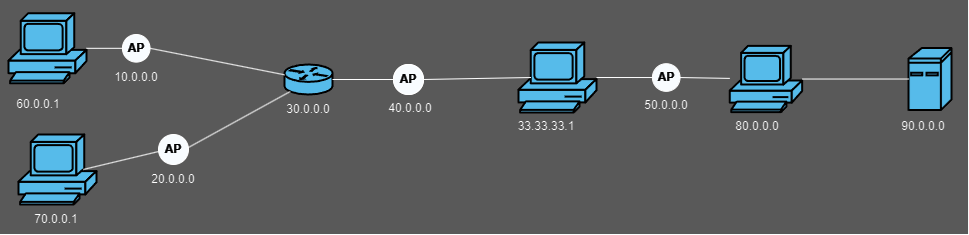
\includegraphics[width=1\textwidth]{EsempioProtection.png}  % Sostituisci 'nome_immagine' con il nome del tuo file immagine e l'estensione
    \caption{Grafo di allocazione d'esempio per requisiti di protezione}
    \label{fig:EsempioProtection}
\end{figure}

In questo esempio, si vuole creare un canale sicuro per far comunicare l'host-S 60.0.0.1 con l'host-D 90.0.0.0. A scopo illustrativo poniamo l'host 33.33.33.1 come nodo non sicuro(untrustedNode)
e l'host 80.0.0.0 come nodo d'ispezione per controllare il traffico in ingresso verso il nodo 90.0.0.0 come se fosse un IDS (inspectorNodes).
Per attuare ciò la definizione da passare in input a Verefoo è la seguente: 

\begin{lstlisting}[style=mystyle,caption={Esempio di requisito di protezione}]
    <PropertyDefinition>
    <Property graph="0" name="ProtectionProperty" src="60.0.0.1"
    dst="90.0.0.0" src_port= "80" dst_port="80">
    <protectionInfo encryptionAlgorithm="AES_128_CBC"
    authenticationAlgorithm="SHA2_256">
    <untrustedNode node="33.33.33.1"/>
    <inspectorNode node= "80.0.0.0"/>
    <securityTechnology>TLS</securityTechnology>
    <securityTechnology>IPSEC</securityTechnology>
    </protectionInfo>
    </Property>
    </PropertyDefinition>
\end{lstlisting}

Una soluzione possibile scelta da Verefoo è la seguente:

\begin{figure}[h]  % 'h' significa che la figura viene posizionata qui
    \centering
    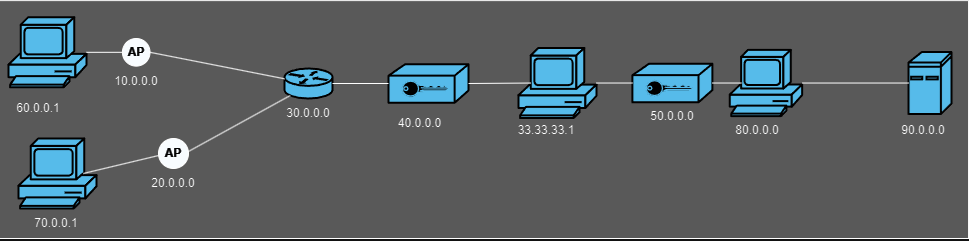
\includegraphics[width=1\textwidth]{ProectionProp.png}  % Sostituisci 'nome_immagine' con il nome del tuo file immagine e l'estensione
    \caption{Output grafo di esempio per requisito di protezione}
    \label{fig:ProtectionRisolta}
\end{figure}

Come si può notare 2 VPN Gateway sono state allocati al fine di garantire i requisiti specificati: il primo al nodo 40.0.0.0
è stato configurato in \textit{"ACCESS MODE"} permettendo a tutti i pacchetti provenienti da 60.0.0.1 e diretti a 90.0.0.0 di entrare nel tunnel VPN, il
secondo invece è stato configurato in \textit{EXIT MODE} così da poter rimuovere la protezione per tutti i pacchetti inserita precedentemente. È inoltre fondamentale
sottolineare come i requisiti che abbiamo richiesto sono stati tutti rispettati. È infatti possibile notare come il nodo considerato non sicuro (33.33.33.1) si trova all'interno del tunnel e ogni
pacchetto che riceve sarà stato precedentemente protetto dal nodo 40.0.0.0. Similmente, il nodo 80.0.0.0 che dovrebbe agire da IDS per la topologia di esempio può svolgere la sua funzione in quanto
tutti i pacchetti in transito vengono precedentemente decifrati dal nodo 50.0.0.0. Infine non avendo specificato alcun collegamento non sicuro verefoo ha garantito soltanto che il collegamento di default
sia sicuro.


\chapter{Docker} \label{ch:docker}

\section{Introduzione a Docker} 

Parte di docker.

\section{Docker Compose}

Parte di Docker compose.

description \cite{noms2020}
\chapter{Conclusions} \label{ch:conclusions}

Conclusion and future works
\bibliographystyle{IEEEtran}
\bibliography{bibliography}
%\include{bibliography}

%if appendixes are needed, uncomment the following lines
%\appendix
%\appendixpage
%\include{appendixA}
%\include{appendixB}



\end{document}

